% SLIDE 1: pagina di presentazione
\frame{\titlepage}

% SLIDE 2: motivazioni
\begin{frame}
    \frametitle{Scenario e Motivazioni}
    Il mondo del Cloud in cooperazione con i sistemi IT ha portato molti benefici, tuttavia vengono sollevate diverse problematiche
    \begin{itemize}
        \item questi sistemi sono spesso \alert{complessi e impegnativi da gestire} se non si hanno conoscenze approfondite in materia, 
        soprattutto per utenti poco esperti
    \end{itemize}
\end{frame}

% SLIDE 3: Moon Cloud
\begin{frame}
    \frametitle{Moon Cloud}
    \begin{columns}
        \begin{column}{0.55\textwidth}
            Moon Cloud è una piattaforma erogata come servizio che supporta un framework di \alert{\textit{Security Assurance}}, 
            basato su politiche di sicurezza definite Controlli ed Evaluation
        \end{column}
        \begin{column}{0.4\textwidth}
            \begin{center}
                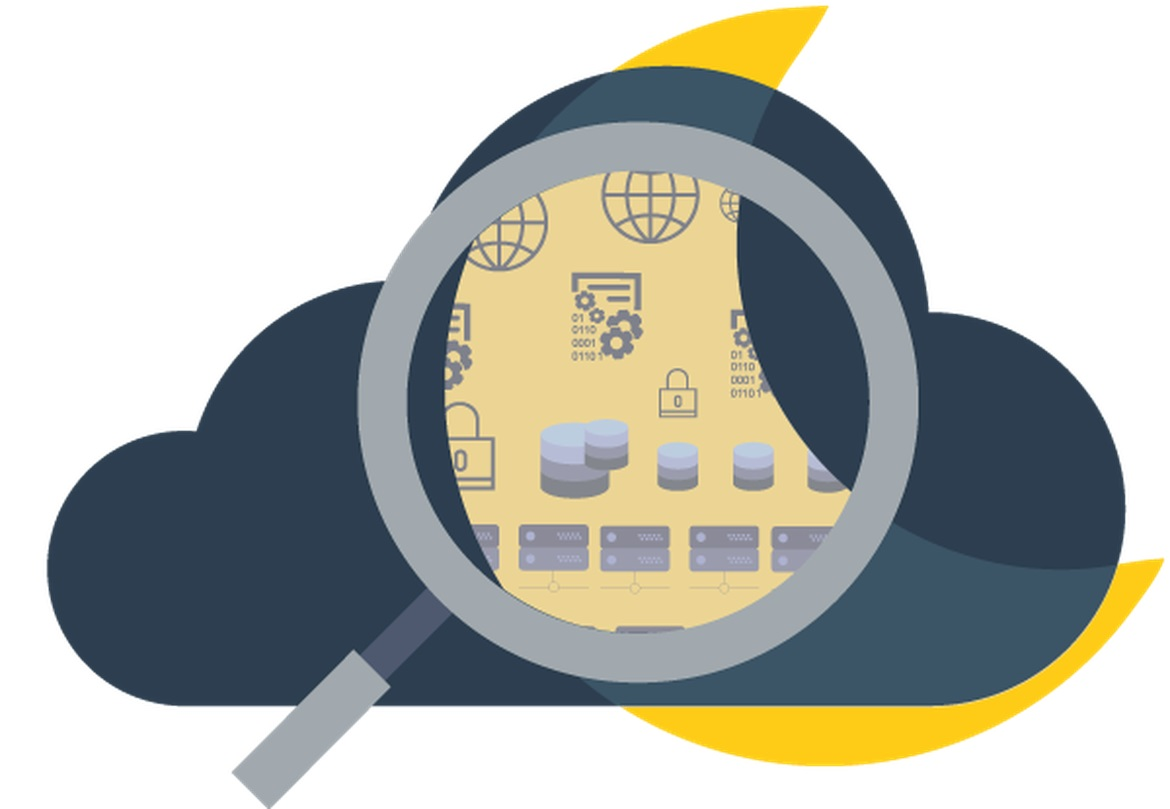
\includegraphics[scale=0.12]{images/mc}
            \end{center}
        \end{column}
    \end{columns}
    Garantisce il controllo della sicurezza informatica in modo rapido ed efficiente, attraverso attività di test e monitoraggio 
    periodiche e programmate
\end{frame}

% SLIDE 4: obiettivo della tesi
\begin{frame}
    \frametitle{Obiettivo della tesi}
    Introduzione di un \alert{sistema di raccomandazione} che possa consigliare all'utente delle possibili \textit{Evaluation} rispetto 
    al \textit{target} che vuole proteggere e monitorare
    \begin{itemize}
        \item l'utente meno esperto può usufruire dei servizi offerti da Moon Cloud in modo \alert{efficace} ed \alert{intuitivo} 
        \item viene supportanto in ogni fase dall'inserimento delle informazioni del target da proteggere fino alla scelta delle 
        attività di monitoraggio da eseguire
    \end{itemize}
\end{frame}

% SLIDE 5: Sistema di Raccomandazione
\begin{frame}
    \frametitle{Sistema di raccomandazione}
    Un \textit{recommendation system} può filtrare i dati usando differenti algoritmi e raccomandare gli item più rilevanti agli utenti attraverso 
    un procedimento a 3 fasi
    \begin{enumerate}
        \item \alert{Raccolta di dati}: ottenere informazioni rilevanti e consistenti su cui applicare algoritmi di raccomandazione
        \item \alert{Memorizzazione di dati}: la quantità di dati definisce quanto efficace un modello di raccomandazione può diventare
        \item \alert{Filtraggio dei dati}: estrarre le informazioni più rilevanti
    \end{enumerate}
\end{frame}

% SLIDE 6: Struttura del database
\begin{frame}
    \frametitle{Struttura base di dati}
    \begin{figure}
        \centering
        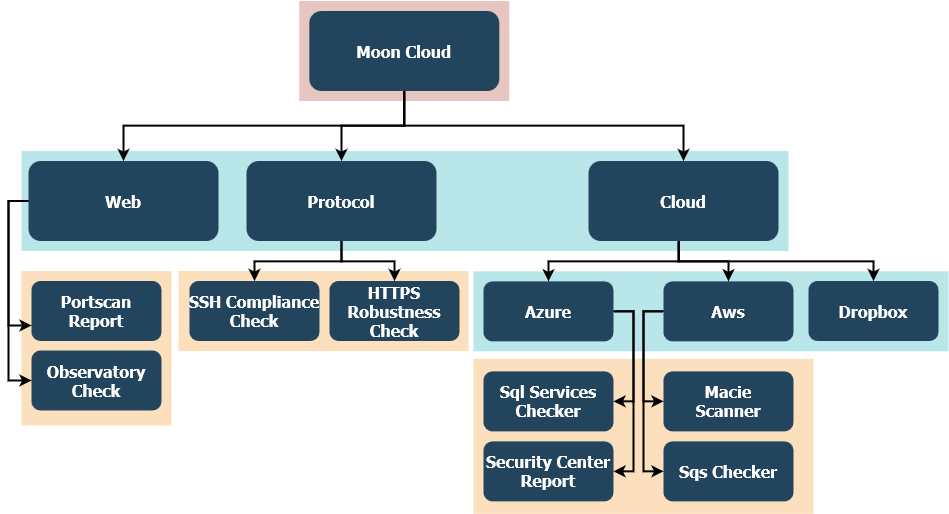
\includegraphics[scale=0.35]{images/MC_Rec_Tree2}
    \end{figure}
\end{frame}

% SLIDE 6: Collaborative Filter
%\begin{frame}
%    \frametitle{Collaborative filtering}
%    Questo sistema predice la preferenza che un utente accorderebbe a un item basandosi sulle preferenze date da altri utenti
%    \begin{itemize}
%        \item \alert{semplici da implementare}, \alert{intuitivi} e non necessitano di operazioni di training sui dati e 
%        regolazione di molti parametri
%        \item permettono all'utente di comprendere le ragioni che si celano dietro ad ogni raccomandazione
%    \end{itemize}
%\end{frame}

% SLIDE 8: Recommendation Algorithms
\begin{frame}
    \frametitle{Recommendation Algorithms}
    \begin{columns}
        \begin{column}{0.5\textwidth}
            \begin{figure}
                \centering
                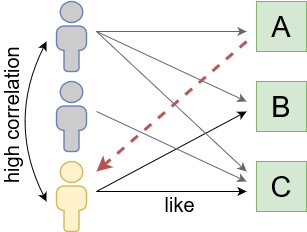
\includegraphics[scale=0.5]{images/UB_CF_ex}
           \end{figure}
           \alert{User Based Collaborative Filter}: algoritmo che fornisce dei suggerimenti sulla base di uno o più vicini (\textit{neighbours}) 
        \end{column}
        \begin{column}{0.5\textwidth}
            \begin{figure}
                \centering
                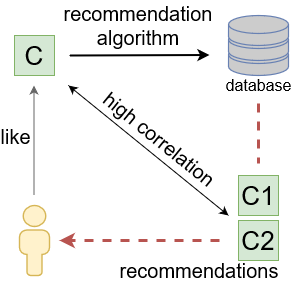
\includegraphics[scale=0.55]{images/IB_CF_ex2}
            \end{figure}
            \alert{Item based Collaborative Filter}: algoritmo che confronta gli item dell'utente a cui si vuole raccomandare e i possibili item simili 
        \end{column}
    \end{columns}
\end{frame}

% SLIDE 9: Soluzione
\begin{frame}
    \frametitle{Soluzione}
    Servizio di \alert{API REST} accessibile attraverso apposite URL che permette di effettuare richieste al sistema di 
    raccomandazione e di mantenere consistente la base di dati
    \begin{itemize}
        \item si possono richiamare diversi algoritmi di raccomandazione
        \begin{itemize}
            \item \alert{algoritmo di raccomandazione User-based}, il quale si basa sulle Evaluation usate dall'utente a cui si vuole raccomandare 
            \item \alert{algoritmo di raccomandazione Item-based}, il quale si può basare o su Evaluation o su Target forniti dall'utente 
            \item \alert{algoritmo di raccomandazione Ibrido}, cerca di mettere insieme i pregi dei precedenti algoritmi per determinare le Evaluation simili
        \end{itemize}
    \end{itemize}
\end{frame}

% SLIDE 9: Soluzione (2)
\begin{frame}
    \frametitle{Soluzione (2)}
    \begin{figure}
        \centering
        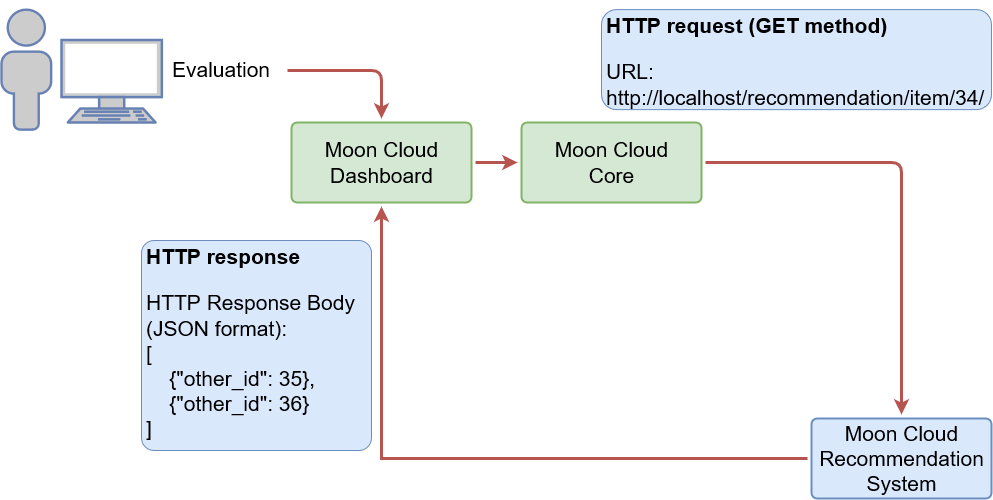
\includegraphics[scale=0.32]{images/UML_MoonCloud_HowToDoPres}
    \end{figure}
\end{frame}

% SLIDE 10: Conclusioni
\begin{frame}
    \frametitle{Conclusioni}
    La soluzione introduce un sistema di raccomandazione in un mondo in cui spesso non è presente perché 
    popolato da utenti esperti
    \begin{itemize}
        \item la configurazione delle attività di test vengono semplificate 
        \item un maggior numero di utenti può fare uso di questi sistemi in totale sicurezza e affidabilità 
    \end{itemize}
\end{frame}
